\chapter{Research}
\label{ch:background}

This chapter provides background context for the development of a liquid democracy system within Vodle. It builds on the concepts introduced earlier, focusing on more detailed research into known limitations of liquid democracy and potential solutions proposed in academic literature. Additionally, the technical foundations and design philosophy of Vodle as a platform are explored.

Throughout this chapter, several diagrams are used to illustrate how votes move through a liquid democracy system. To clarify the roles of different voters, the following symbols are used:
\begin{itemize}
    \item \textbf{Circles} indicate voters who delegate their vote to someone else.
    \item \textbf{Squares} represent voters who cast their own vote and do not delegate.
    \item \textbf{Triangles} show voters who abstain - neither voting directly nor delegating to others.
\end{itemize}

\section{Liquid Democracy}

Liquid democracy, or delegative voting, allows voters to either cast a vote directly, delegate it to someone they trust, or abstain \citep{blum_liquid_2016}. A key feature is that delegations are transitive - a chain of users that all delegate to each other sequentially ends with a single final voter who casts their vote on behalf of all those in the chain.

Whilst the transitivity property enables concentration of voting power with trusted individuals, it can also lead to unintended consequences. Chains of delegations may result in cycles that prevent votes from being cast, or allow certain individuals to accumulate an excessive share of influence, creating so-called super-voters. These problems amongst others motivate the need for alternative delegation mechanisms, as discussed in the following subsections.

%\cite{ford_delegative_2002} argues that direct democracy becomes ineffective at scale due to the diversity in participants' knowledge and interest. Without mechanisms to channel influence through trusted intermediaries, the collective outcome may reflect average rather than informed decision-making. Liquid democracy addresses this by enabling voters to shift influence toward participants with greater expertise or engagement.

\subsection{Issues with Liquid Democracy}

\subsubsection{Delegation cycles}
\begin{figure}[h]
    \centering
    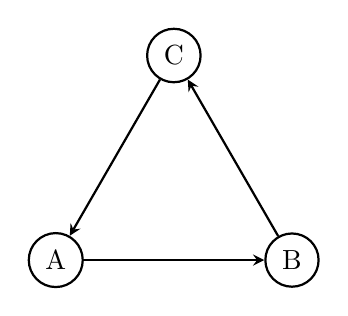
\begin{tikzpicture}[->, >=stealth, thick, scale=1.5]
        % Nodes at triangle vertices
        \node[circle, draw] (A) at (0,0) {A};
        \node[circle, draw] (B) at (2,0) {B};
        \node[circle, draw] (C) at (1,1.732) {C}; % height = sqrt(3)

        % Arrows showing delegation
        \draw (A) -- (B);
        \draw (B) -- (C);
        \draw (C) -- (A);
    \end{tikzpicture}
    \caption{Delegation cycle: A delegates to B, B to C, and C back to A.}
    \label{fig:triangle-cycle}
\end{figure}


Delegation cycles occur when a vote is delegated in such a way that it ends up forming a loop \citep{brill_liquid_2022}, preventing the vote from reaching a final, resolvable destination. For example, if Alice delegates her vote to Bob, Bob delegates to Charlie, and Charlie delegates back to Alice, the votes become trapped in a cycle (seen above) and can be treated as a loss of representation \citep{christoff2017liquiddemocracyanalysisbinary}.

This issue is particularly problematic because it can nullify votes without the affected users ever realising. In systems where cycles are not explicitly detected and handled, these votes are discarded silently, potentially changing the final outcome of the votes.

Delegation cycles are increasingly likely to emerge in dynamic voting systems, where delegations can be added, removed, or modified at any point in time. Delegations that initially did not form part of a cycle may later contribute to one as other voters add a new delegation or alter an existing one.

\textit{Paragraph on how size of the system affects the possibility of cycles?}

\subsubsection{Abstentions}
\begin{figure}[h]
    \centering
    \begin{tikzpicture}[->, >=stealth, thick, node distance=2.5cm]
        \node[circle, draw] (A) {A};
        \node[circle, draw, right of=A] (B) {B};
        \node[regular polygon, regular polygon sides=3, shape border rotate=0, draw, minimum size=1cm, inner sep=0pt, right of=B] (C) {C};

        \draw (A) -- (B);
        \draw (B) -- (C);
    \end{tikzpicture}
    \caption{Delegation chain ending in abstention: A delegates to B, B to C. C abstains, causing the votes of A and B to be lost.}
    \label{fig:delegation-abstention}
\end{figure}

In liquid democracy, abstention is where a voter neither casts a vote nor delegates their vote to another user \citep{brill_liquid_2022}. This includes both deliberate abstention, where a voter knowingly chooses not to participate, and passive abstention, where a voter may be unaware of an ongoing poll or are unable to engage with it.

Abstentions are especially impactful when they occur at the end of a larger delegation chain, as all votes passed along the chain to that voter are effectively lost \citep{brill_liquid_2022}. The voters whose decisions were passed along the chain may also be unaware that their votes have been nullified, worsening the effect of the abstention.

\subsubsection{Super-voters}
In liquid democracy, a super-voter is an individual who receives a large number of delegated votes, therefore gaining disproportionate influence over decisions \citep{kling2015votingbehaviourpoweronline}. While this behaviour may reflect voters' genuine preferences, it can lead to a concentration of power that goes against the intended egalitarianism and democratic ideals of liquid democracy.

Although liquid democracy allows users to alter their delegation at any time, in practice, many voters may not actively monitor or even know how their vote is being used. This can allow a small number of super-voters to dominate outcomes, especially in systems with large delegation chains.

Real-world examples of this phenomenon have been documented. In the German Pirate Party's use of LiquidFeedback, certain users received so many delegations that their votes were like ``decrees'' \citep{sven_becker_liquid_2012,kling2015votingbehaviourpoweronline} even though they were not elected officials. \cite{kling2015votingbehaviourpoweronline} noted that the super-voters generally voted in line with the majority, therefore not drastically affecting the outcome of the votes and contributed to the stability of the system. However, the potential for individuals to single-handedly influence the results remained a concern.
%This pattern has also been observed in blockchain-based governance systems \citep{hallWhatHappensWhen2024}, where voting tokens (digital representations of voting power) are commonly concentrated among a few delegates, giving them an excessive amount of power.
%In the case of the Pirate Party, analysis showed that although super-voters held significant theoretical power, they generally voted in line with the majority, therefore not drastically affecting the outcome of the votes. \cite{kling2015votingbehaviourpoweronline} described this behaviour as voting "wisely," noting that while these individuals had the capacity to change outcomes, they typically did not use it to push their own agenda.

This pattern is not limited to traditional online voting platforms. It can also be seen within decentralised autonomous organisations (DAOs) - blockchain-based entities where decisions are made collectively by token holders without central leadership. These organisations use token-based voting to decide on critical issues like protocol upgrades and funding allocations. \cite{hallWhatHappensWhen2024} studied 18 decentralised autonomous organisations (DAOs) and found that voting power was often concentrated in the hands of a few delegates. While most did not control a large share of all available tokens, low participation meant that their share of actual votes cast was disproportionately high. In several DAOs, the top five delegates accounted for over 50\% of all votes cast, and in the DAO Gitcoin, this figure exceeded 90\%.

\subsection{Variations of Liquid Democracy}
The challenges discussed in the previous section, such as delegation cycles, vote loss due to abstentions, and the emergence of super-voters, highlight inherent vulnerabilities in the standard liquid democracy model. To mitigate these issues, a range of enhancements have been proposed that modify how delegations are expressed, resolved, or overridden. These include techniques that allow voters to specify multiple delegates or distribute their vote to multiple casting voters. Each approach introduces different trade-offs and requires algorithmic support to ensure sound and interpretable outcomes.

The following subsections present several such variations, along with the algorithms that support them.
\subsubsection{Ranked Delegation}
One way to improve the reliability of liquid democracy is through ranked delegation. Instead of selecting a single delegate, voters can provide an ordered list of trusted individuals. If a higher-ranked delegate cannot cast the vote, due to abstaining, becoming part of a cycle, or being otherwise unavailable, the system attempts to use the next delegate in the list. This structure increases the chance that votes are not lost while preserving the core interaction model for voters \citep{brill_liquid_2022}.

To implement ranked delegation, the system must determine which delegation path to follow when multiple options are available. This is achieved using a delegation rule - a function that takes as input a ranked delegation instance and a delegative voter and outputs a path from that voter to a casting voter (a voter that does not delegate or abstain, casting their own vote) \citep{brill_liquid_2022}.

Several rules have been proposed in the literature, each with distinct properties and trade-offs.

Before examining these rules, it is useful to outline several properties that are commonly used to evaluate them:

\textbf{Guru participation} ensures that a voter who accepts delegated votes (a guru) is never disadvantaged by doing so. That is, receiving additional delegations should not reduce their influence over the outcome \citep{kotsialou_riley_2020}.

\textbf{Confluence} requires that each voter have a single, unambiguous delegation path. This property simplifies the resolution of delegations and enhances system transparency \citep{brill_liquid_2022}.

\textbf{Copy robustness} aims to prevent a specific form of strategic manipulation which occurs when a voter who would normally delegate decides to act as a casting voter and mimics the behaviour of their delegate outside the system (for example, by copying their vote using external communication). In non-copy-robust systems, this behaviour can result in a greater combined influence for both the original delegate and the copier, effectively bypassing the system. A copy-robust rule avoids this problem by ensuring that the combined voting weight of the mimicked behaviour does not exceed what it would have been through proper delegation \citep{brill_liquid_2022,behrens_2015}, giving equal opportunities to all voters.

The main delegation rules that were considered for implementation are:

\textbf{Depth-First Delegation (DFD)} selects the path with the highest-ranked first delegate, even if it results in a long chain. While this rule prioritises individual trust rankings, it fails to satisfy the \textit{guru participation} property, as show by \cite{kotsialou_riley_2020}.

\textbf{Breadth-First Delegation (BFD)} prioritises the shortest available delegation path and uses rankings only to resolve ties. This approach generally results in more direct and predictable delegation chains and satisfies \textit{guru participation} \citep{kotsialou_riley_2020, brill_liquid_2022}, though it may assign votes to lower-ranked delegates.

\textbf{MinSum} strikes a balance between path length and preference by selecting the path with the lowest total sum of edge ranks. This rule is \textit{confluent} and helps avoid both long chains and poorly ranked delegations, making it suitable for general use \citep{brill_liquid_2022}.

\textbf{Diffusion} builds delegation paths in stages, assigning votes layer by layer based on the lowest available rank at each step. This approach avoids poor delegations but can occasionally produce unintuitive results due to its tie-breaking method \citep{brill_liquid_2022, colley_smart_2020}.

\textbf{Leximax} addresses this by comparing delegation paths based on their worst-ranked edge. It ensures that poorly ranked delegations are avoided, especially near the beginning of a path, and maintains the \textit{confluence} property \citep{brill_liquid_2022}.

\textbf{BordaBranching} takes a global view of the delegation graph and selects a branching that minimises the total rank across all delegation edges. It satisfies both \textit{guru participation} and \textit{copy robustness}, making it well-suited for robust and equitable systems \citep{brill_liquid_2022}. However, this rule can be computationally intensive to implement.

In summary, ranked delegation significantly improves the reliability of liquid democracy, as it results in a lower chance of a delegated vote being nullified. The choice of delegation rule influences not only system efficiency but also the fairness of outcomes. While simpler methods such as DFD and BFD are easier to implement, advanced rules like MinSum, Leximax, and BordaBranching offer stronger guarantees and are better suited to practical deployment in platforms such as vodle.

\subsubsection{Weighted/ vote splitting}
Voting power is distributed across multiple delegates to reduce reliance on any single individual (\cite{golz_fluid_2021}).

\section{Implementations of Liquid Democracy}
\subsection{LiquidFeedback}
\subsection{Google Votes}

\section{vodle}
Vodle is a web-based platform for participatory group decision-making. Users participate in polls that allow them to rate a set of options using sliders. When the poll ends, these ratings are aggregated and the MaxParC rating system is used to determine the final result of the poll.

\subsection{MaxParC}
Understanding MaxParC is important for this project because it forms the core of how vodle interprets group preferences. Since this work involves modifying vodle's voting behaviour through the integration of liquid democracy, it is essential to understand how MaxParC processes input ratings. In particular, understanding how changes in individual ratings influence the final outcome of a poll helps to frame the implications of delegating or reweighting votes.
%A clear grasp of MaxParC's underlying principles allows for a more informed and effective integration that maintains the platform's commitment to fairness and consensus.

Maximum Partial Consensus (MaxParC), the rating system used by vodle, was introduced by \cite{heitzig_fair_2024}. It is a decision-making method designed to address the limitations of traditional voting systems, in particular the potential for majority rule to suppress minority viewpoints.
The primary objective of MaxParC is to achieve a balance between fairness, consensus, and efficiency in group decision-making.

Each voter rates an option from $0$ to $100$ ($x$), representing their willingness to approve that option if and only if $<x\%$ of users do not approve that option. Therefore, a rating of $0$ means ``do no approve no matter what'' and a rating of $100$ means ``approve no matter what'' or ``always approve''.

\subsection{Architecture}

\subsubsection{Technologies Used}
why info is relevant to the project - e.g. need to jsonify data. what makes angular different etc
\subsection{Design Philosophy}

\section{Summary}


